\scanpage{81}

$f$ fonction convexe sur l'ouvert convexe $U$,

\[
(x,y)\in G_f\iff x\in U\text{ et } y>f(x)
\]

Soit \deleted{\unsure{$x_0,y_0$|$x,y$|$x_i,y_i$}} $(a,b)$ avec $b=f(a)$ $(a\in U)$, \deleted{\unsure{donc|on}} soit $H$ un hyperplan passant par $(a,b)$ ne rencontrant pas l'ouvert $G_f$, alors : 1) il est de la forme

\[
y-b=\deleted{\unsure{\sum c_i x_i+\beta}}=\sum c_i(x_i-a_i)
\]

(car ne contient pas la droite $x=a$), soit $y=L_a(x)$

2) On a $f(x)\geq L(x)$ pour \uline{\unsure{tout|tt}} $x\in U$ (en effet, l'un des deux \deleted{\unsure{hyperplans}} $\frac12$ espaces \inserted{ouverts} déterminés par $H$ contient $G_f$, et ce ne peut-être que celui donné par $y\geq L(x)$. \deleted{\unsure{donc}} d'où la conclusion), 3) On a pour $x\in E$ $f(x)=\sup_a L_a(x)$ (le sup étant obtenu), et réciproquement. 4) Si au point $a$, $f(x)$ est croissante alors les $c_i$ sont $\geq0$. En effet, si on avait p. ex $c_1<0$, alors $f(x_1,a_2,-a_n)$ est croissante au point $x_1=a_1$,
\reversemarginpar\margin{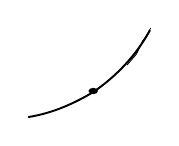
\begin{tikzpicture}[x=.1mm,y=-.1mm,line cap=round,line join=round]
\draw[line width=.7pt] (11,122) .. controls (42,117) and (68,105) .. (92,91) .. controls (122,71) and (148,43) .. (165,12);
\draw[line width=.25pt] (81,97) .. controls (105,84) and (129,63) .. (148,40) -- (166,9);
\draw[line width=.3pt] (136,56) -- (148,42) -- (156,25) -- (162,18);
\fill (93,89) ellipse (6 and 4);
\end{tikzpicture}}\normalmarginpar
et \deleted{de} minorée par $L(x_1,a_2-a_n)$, fonction linéaire prenant au \unsure{pt|point} $a$ la $=$ valeur que $f$. Cette dernière ne peut être strictement décroissante car on aurait $f(x_1)\leq f(a)\leq f(x_1)$ pour $x_1<a_1$ voisin de $a_1$.

\reversemarginpar\margin{82}\normalmarginpar
